%
% File acl2014.tex
%
% Contact: koller@ling.uni-potsdam.de, yusuke@nii.ac.jp
%%
%% Based on the style files for ACL-2013, which were, in turn,
%% Based on the style files for ACL-2012, which were, in turn,
%% based on the style files for ACL-2011, which were, in turn, 
%% based on the style files for ACL-2010, which were, in turn, 
%% based on the style files for ACL-IJCNLP-2009, which were, in turn,
%% based on the style files for EACL-2009 and IJCNLP-2008...

%% Based on the style files for EACL 2006 by 
%%e.agirre@ehu.es or Sergi.Balari@uab.es
%% and that of ACL 08 by Joakim Nivre and Noah Smith

\documentclass[11pt]{article}
\usepackage{paper}
\usepackage{times}
\usepackage{algorithm}
\usepackage{algpseudocode}
\usepackage{multirow}
\usepackage{url}
\usepackage{latexsym}
\usepackage[utf8]{inputenc}
\usepackage{graphicx}
\usepackage{color}

%\setlength\titlebox{5cm}

% You can expand the titlebox if you need extra space
% to show all the authors. Please do not make the titlebox
% smaller than 5cm (the original size); we will check this
% in the camera-ready version and ask you to change it back.


\title{Selección de Instancias}

\author{Formica, Gabriel\\
  Universidad Simón Bolívar\\
  Caracas, Venezuela\\
  {gabrielformica93@gmail.com} \\\And
  Ponte, José Antonio\\
  Universidad Simón Bolívar\\
  Caracas, Venezuela\\
  {pontezambrano@gmail.com} \\}

\date{}

\begin{document}
\maketitle
\begin{abstract}
  El problema de \textit{Selección de Instancias} (IS por sus siglas en inglés), busca
  escoger un subconjunto de instancias de menor cardinalidad del conjunto original
  que mantenga o mejore la clasificación de las muestras a ser usadas como un conjunto
  de entrenamiento. En este articulo se considera la resolución de este problema
  mediante varios algoritmos metaheurísticos, finalizando con los resultados 
  experimentales y comparaciones entre ellos.
\end{abstract}

\section{Definición del Problema}

Un conjunto de datos se define en función de un conjunto de clases $\Omega$ y
un conjunto de $n$ observaciones $T$. Un problema de SI se define entonces como dicho 
conjunto de instancias 
$T = \{t_{1}, t_{2},..., t_{n}\}$, donde una instancia (observación) $t_{i}$ es
una tupla $t_{i} = (v_{i,1}, v_{i,2},...,v_{i,m})$ de $m$ valores/mediciones
(un punto en un espacio m-dimensional). Además, cada instancia $t_{i}$
pertenece a una clase $w_{t_{i}}  \epsilon  \Omega$. 

La idea es seleccionar un subconjuto de menor cardinalidad 
$R \subseteq T$ tal que $R$ mantega o mejore la capacidad 
de representación del conjunto $T$.

\section{Descripción de la solución}

En esta sección se muestra al lector el proceso de construcción de una 
solución. Especificamente, se muestra cómo se representa una solución,
cómo se generan las soluciones iniciales, y finalmente, se incluye 
el pseudocódigo de la metaheurística implementada.

\subsection{Representación}

Sea un conjunto inicial $T$, una solución al problema de SI está
dado por un subconjuto de instancias $R$,
que puede ser fácilmente representado por una cadena de bits de 
tamaño $n = |T|$ donde cada bit tiene valor 1/0, indicando respectivamente,
la pertenencia o no de una instancia $t_{i} \epsilon T$ en la solución. 

\subsection{Generación de soluciones iniciales}

Siendo una representación una cadena de bits, para generar una solución
inicial seguimos una estrategia muy sencilla: cada bit tiene una probabilidad $\rho$
de estar en la solución. Si bien en la literatura, lo común es
que $\rho$ sea igual a $0.5$, de manera de comenzar con un solución
de $50\%$, en nuestro caso hemos hecho varias ``corridas'' con distintos valores
de $\rho$, generando soluciones iniciales de distintos tamaños, de manera de poder
evaluar el impacto de cada una de estas reducciones.

\section{Función de evaluación}
En (Cano et. al 2003) se describe una función de evaluación que considera la tasa de instancias clasificadas correctamente tomando en cuenta el conjunto reducido como conjunto de entrenamiento y una tasa de reducción del conjunto original. Se hace uso de una constante $\alpha$ donde $\alpha \in [0,1]$ para darle ponderación a ambos parámetros. La fórmula usada para medir la calidad de una solución es:

~\

\begin{center}
    {\fontsize{10}{10}\selectfont
    $ evaluar(R) = \alpha \times tasa\_clas + (1 - \alpha) \times porcen\_redc $
    }
\end{center}

~\

El objetivo de un algoritmo es maximizar esta función, entonces si $evaluar(A) < evaluar(B)$, se tiene que $B$ es mejor solución que $A$. Para los experimentos se usó la tasa sugerida por (Cano et. al 2003) de $\alpha = 0.5$ dándole la misma ponderación a $tasa\_clas$ y a $porcen\_redc$.

\section{Algoritmos}

    \subsection{Búsqueda local}
    Para la búsqueda local se hace uso de un algoritmo inspirado en \emph{hill-climbing} el cual toma una solución inicial y tiene como objetivo mejorarla haciendo uso de un operador $op: S \to S$. \\

    {\fontsize{10}{10}\selectfont
    \begin{algorithmic}
        \Function{BusquedaLocal}{$T: Problema$}
            \State $S \gets solucionAleatoria()$
            \While{$\lnot condicionDeParada$}
                \State $R \gets S$
                \State $R \gets operador(R)$
                \If{\Call{calidad}{R,T} $<$ \Call{calidad}{S,T}}
                    \State $S \gets R$
                \EndIf
            \EndWhile
            \State return $S$
        \EndFunction
    \end{algorithmic}
    }

    ~\ 

    Como condición de parada se establece que el mínimo de calidad de una solución sea $0.95$ y una cantidad determinada de iteraciones en las cuales la solución no cambie.

\subsection{1NN}
    Para el cálculo de la calidad de una solución, se hace uso del clasificador $1NN$ que clasifica un conjunto usando un conjunto definido como entrenamiento. Sobre los resultados obtenidos de $1NN$ se corre una función de evaluación que asinga un valor a la solución. \\

    {\fontsize{10}{10}\selectfont
    \begin{algorithmic}
        \Function{Calidad}{$S: Solucion$, $T: Problema$}
            \State $Problema$  $entrenamiento$
            \State $Problema$  $resultado$
            \State $resultado \gets \Call{1NN}{entrenamiento, T}$
            \State $retorna$ $eval(resultado)$
        \EndFunction
    \end{algorithmic}
    }


\subsection{Operador}
Ante la necesidad de movernos en el
espacio de busqueda, surge la idea de un operador 
que modifique de manera sutil (y rápida) una solución
dada. 
En nuestro caso, nuestro operador selecciona al
azar un bit ``prendido'' y lo ``apaga'', que se traduce
en ``sacar'' una instancia del conjunto de instancias solución.

De esta manera, se consiguen soluciones cada vez más pequeñas y una tasa
de aciertos $tasa\_clas$ cada vez más precisas: esto viene de si tenemos 
$x$ aciertos y $w$ instancias que no están en la solución, aumetar el tamaño
de una solución conllevaría a una posible $tasa\_clas = x / (w - 1) $,
que supondría una mayor $tasa\_clas$ y por lo tanto una mejor solución. Sin embargo, 
esto no puede estar más alejado de la realidad.


\section{Experimentos}

Se seleccionaron instancias de tamaño pequeño con menos de 1000 instancias y mediano con más de 1000 pero menos de 5000 instancias. Cada problema cuenta con atributos y clases en el dominio de los reales.

\subsection{Resultados}
 
 Se seleccionan tres casos pequeños y se observa que el porcentaje de reducción es pequeño.

\begin{table}[h]
\begin{tabular}{ |l|l|l|l| }
    \hline
    Caso & Instancias & Atributos & \% red. \\ \hline
    Haberman & 306 & 4 & 13.7 \\ \hline
    Heart & 270 & 14 & 46 \\ \hline
    Fertility & 100 & 10 & 34 \\ \hline
\end{tabular}
\caption{Datos pequeños}
\label{tabla:1}
\end{table}

    ~\

    Para los casos medianos, se observa que el porcentaje de reducción es mucho mayor

    ~\

\begin{table}[h]
\begin{tabular}{ |l|l|l|l| }
    \hline
    Caso & Instancias & Atributos & \% red. \\ \hline
    Phishing & 2456 & 31 & 84 \\ \hline
    Segment & 2310 & 20 & 87 \\ \hline
    Bank & 1372 & 5 & 90 \\ \hline
\end{tabular}
\caption{Datos medianos}
\label{tabla:2}
\end{table}

\subsection{Entonación}

Cada metaheuística se comporta de manera distinta. Entonar 
los parametros de cada una de ellas requirió de una serie 
de pruebas sobre distintos problemas, parametrizando
no solo dichos valores, sino hasta operadores de vencindad. 
Por ejemplo, \emph{Simulated Annealing}, arrojaba mejores 
resultados a medida que mayor era la \emph{temperatura} y menor el \emph{factor de decrecimiento},
y usando como operador de vencidad \emph{percRandomFlips} con $5\%$. Sin embargo,
aumentar la temperatura y disminuir el factor de decrecimiento implica ejecuciones 
de mayor tiempo (mayor
diversificación). Es por esto que para los resultados finales, se consideró $temperatura = 15.000$ 
y $factor = 1$, obteniendo así un equilibrio entre el tiempo de ejecución y calidad de la solución. 


\subsection{Comparación}

Una vez decididos los parametros de cada metaheurística, se realizaron 
hasta 15 pruebas con cada una de ellas en \emph{Glass}. Los gráficos 
presentes sugieren que \emph{ILS} es la que mejor que se comporta para este problema, 
tanto en promedio del tamaño de la solución final (\% del conjunto de instancias), 
como en porcentaje de errores sobre el conjunto de validación.

\begin{center}
  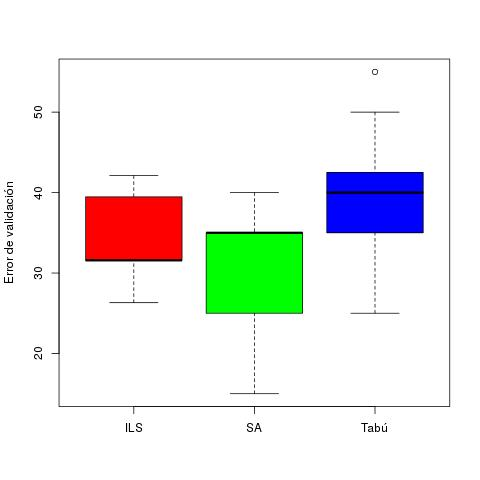
\includegraphics[scale=0.4]{val_errors.jpeg}~\\[1cm]
\end{center}

\begin{center}
  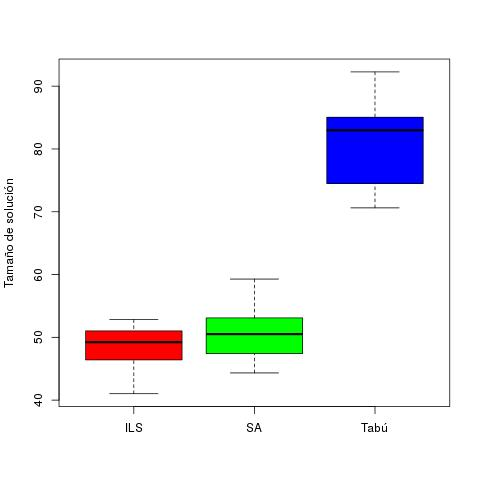
\includegraphics[scale=0.4]{sizes.jpeg}~\\[1cm]
\end{center}





% include your own bib file like this:
%\bibliographystyle{acl}
%\bibliography{acl2014}

\begin{thebibliography}{}

\bibitem[\protect\citename{Cano et al}2003]{Cano:03}
José Ramón Cano, Francisco Herrera, and Manuel Lozano.
\newblock 2003.
\newblock {\em Using evo-
lutionary algorithms as instance selection for data reduction in kdd: an
experimental study.}.
\newblock Evolutionary Computation, IEEE Transactions.

\bibitem[\protect\citename{Toussaint}200]{Toussaint:02}
Godfried Toussaing.
\newblock 2002.
\newblock {\em Proximity Graphs for Nearest Neighbor Decision Problem}.
\newblock School of computer science. McGill University

\end{thebibliography}

\end{document}
